\chapter{Theoretical Background}\label{chap:01}

\section{LHCb}

\begin{figure}[H]
    \centering
    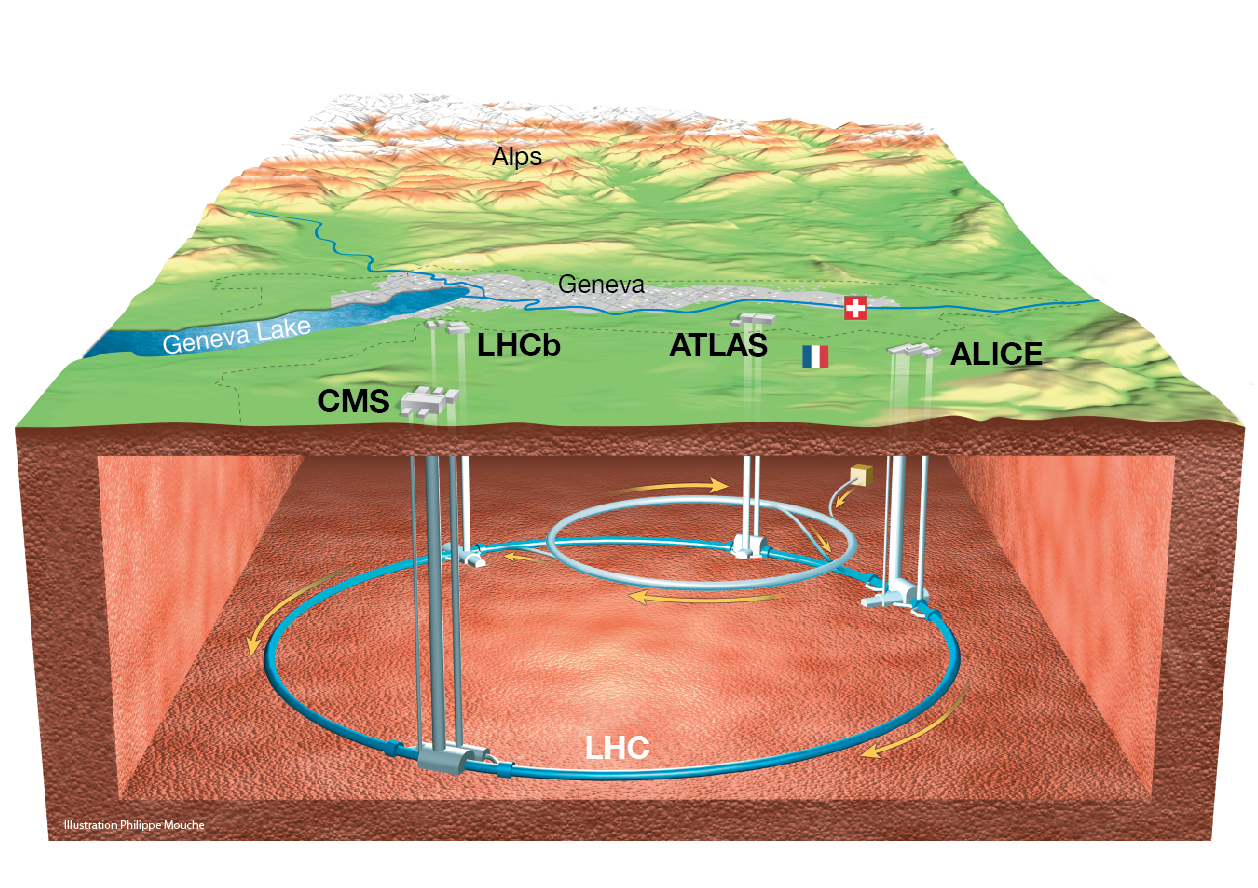
\includegraphics[width=0.7\linewidth]{images/LHC_scheme.png}
    \caption{LHC schema with ALICE, Atlas, CMS and LHCb at CERN.}
    \label{LHC}
\end{figure}

The LHCb Detector is part of one of the four large experiments set up on different points of the circular accelerator design of LHC, at CERN. Our detectors are constructed around collision points where the accelerated beams of protons are crossed with each other \( 40 \times 10^{16} \) times per second. Unlike rest of the detectors at LHC, the LHCb detector is built to detect particles from a singular direction, with the official name for the design being, "Single arm forward spectrometer". It can detect particles coming from the interaction point in the pseudorapidity range between 2 < η < 5 and it is design philosophy is geared towards measuring b (bottom) and c (charm) hadron properties alongside CP violation. \cite{LHCb_detector}


\begin{figure}[H]
    \centering
    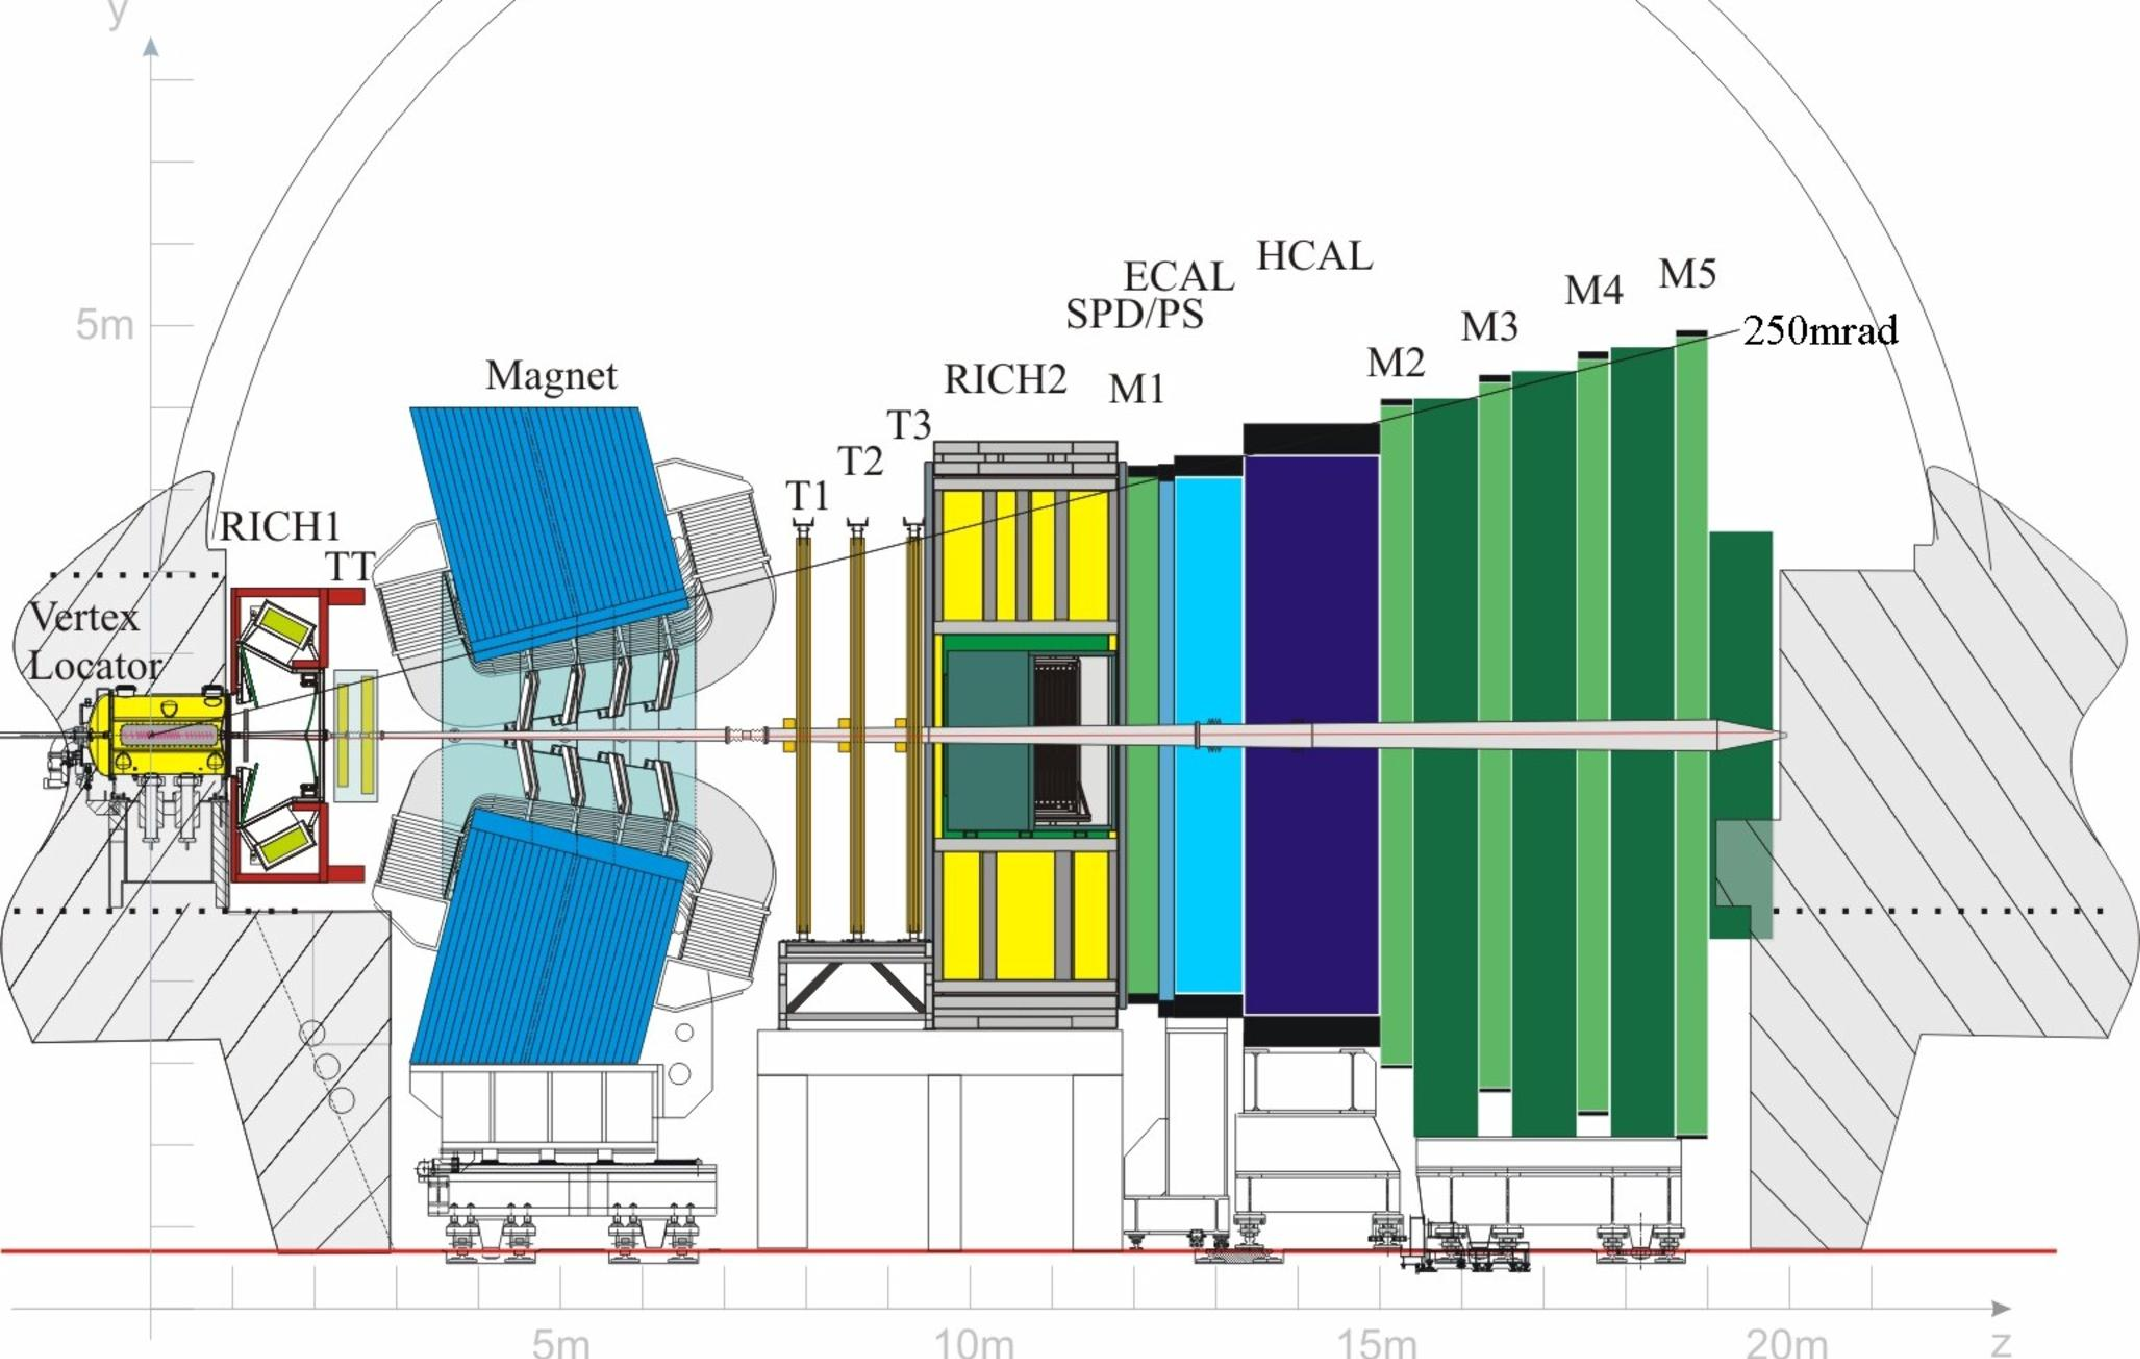
\includegraphics[width=0.7\linewidth]{images/LHCb_diagram.png}
    \caption{The LHCb Detector.}
    \label{LHCb}
\end{figure}

(Detector elements from left to right:  I-Vertex locator, II-Ring Imaging Cherenkov Detector 1, III-Trigger Tracker(TT), IV-Dipole Magnet, V-Outer Trackers(T1,T2 and T3), VI-Ring Imaging Cherenkov Detector 2, VII-Muon Detector 1, VIII-Electromagnetic and Hadronic Calorimeters, IX-Muon Detector 2,3,4 and 5).

The LHCb detector is made up of the following components:
%--------------%
\begin{enumerate}[label=\textbf{\arabic*.}]
    \item \textbf{VELO (Vertex Locator)}
    
    \textbf{Purpose:} Precise reconstruction of primary and secondary vertices coming from the collision.
    
    \textbf{Features:} Silicon-strip detectors close to the beam line, retractable during the beam injection phase.
%--------------%
    \item \textbf{TT Station (Trigger Tracker)}
    
    \textbf{Purpose:} Tracking particles before entering the magnetic field.
    
    \textbf{Features:} Silicon microstrip detector upstream of the magnet.
%--------------%
    \item \textbf{Dipole Magnet}
    
    \textbf{Purpose:} Bends charged particles, making it possible to measure their momentum later.
        
    \textbf{Features:} Approximately 4 T$\cdot$m integrated Magnetic field special to the forward spectrometer design.
%--------------%
    \item \textbf{Tracking Stations (T1,T2 and T3)}
    
    \textbf{Purpose:} Tracking particles after leaving the magnetic field (Tracking charged particles for momentum measurement.).
    
    \textbf{Features:} Straw tube drift chambers that cover a large radius.
%--------------%
    \item \textbf{RICH Detectors (Ring-Imaging Cherenkov Detectors)}
    
    \textbf{Purpose:} Particle identification (separating pions, kaons, protons).
    
    \textbf{Features:} Based on the Cherenkov effect, can measure the velocity of the passing particles by recording the angle of which their Cherenkov radiation is received. The equation for the angle in terms of the velocity of the radiating particle is:
    \[
    \cos(\theta_{C}) = \frac{1}{n \frac{v}{c}} = \frac{c}{n v}
    \]
    where the \qq{$n$} is the refractive index of the detector material.
    \begin{figure}[H]
        \centering
        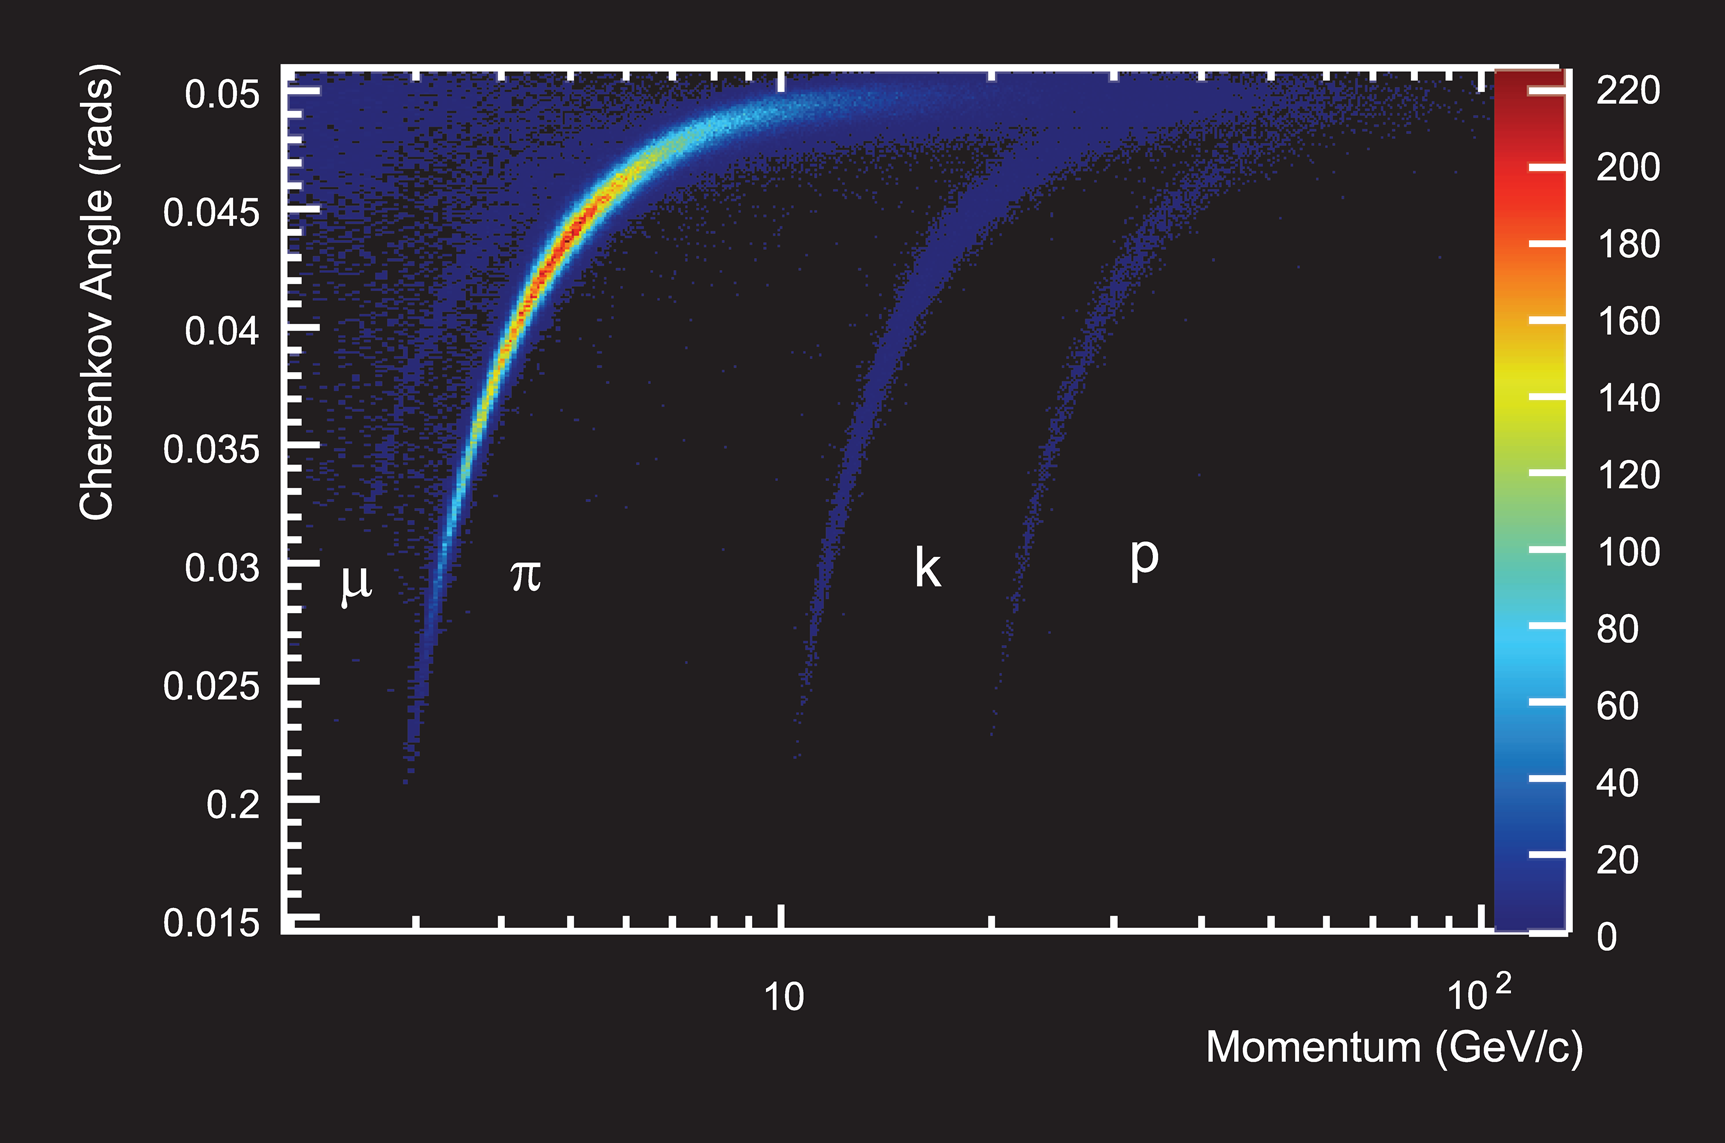
\includegraphics[width=0.59\linewidth]{images/RICH_ID.png}
        \caption{Possible particles and their momentum via a given Cherenkov angle.}
        \label{RICH}
    \end{figure}
%--------------%
    \item \textbf{Calorimeters}
    
    \textbf{Purpose:} Measuring the energy of electrons, photons, and hadrons via particle shower.
    
    \textbf{Features:}
    \begin{itemize}
        \item \textbf{Scintillating Pad Detector:} Electron/photon Identification.
        \item \textbf{Preshower Detector:} Distinguishes electrons from hadrons.
        \item \textbf{Electromagnetic Calorimeter:} Measures energy of electrons and photons.
        \item \textbf{Hadronic Calorimeter:} Measures energy of hadrons (neutral hadrons like neutrons are primarily stopped here).
    \end{itemize}
%--------------%
    \item \textbf{Muon System}
    
    \textbf{Purpose:} Muon identification.
    
    \textbf{Features:} Five stations (M1–M5) using Multi-wire proportional chambers and gas-electron multipliers. The M1 station is before the calorimeters and M2 to M5 after, with shielding in between.
\end{enumerate}

\section{\texorpdfstring{Isolating the $B_{s}^{0}$}{} Decay}

In this lab, we are interested in analysing the specific decay $B_s^0 \rightarrow \psi(2S)\,K_S^0$.
\begin{figure}[H]
    \centering
    \begin{tikzpicture}
        \begin{feynman}
            \vertex (a1) {\(\overline b\)};
            \vertex[right=1.5cm of a1] (a2);
            \vertex[right=1cm of a2] (a3);
            \vertex[right=1.5cm of a3] (a4) {\(\overline d\)};
            \vertex[below=2em of a1] (b1) {\(s\)};
            \vertex[below=2em of a4] (b2) {\(s\)};
            \vertex[above=2em of a4] (c1) {\(c\)};
            \vertex[above=2em of c1] (c2) {\(\overline c\)};
            \diagram* {
            (a4) -- [fermion] (a3) -- [boson, edge label=\(W^{+}\)] (a2) -- [fermion] (a1),
            (b1) -- [fermion] (b2),
            (c2) -- [fermion] (a2),
            (a3) -- [fermion] (c1),
            };
            \draw [decoration={brace}, decorate] (b1.south west) -- (a1.north west)
            node [pos=0.5, left] {\(B^{0}_{s}\)};
            \draw [decoration={brace}, decorate] (c2.north east) -- (c1.south east)
            node [pos=0.5, right] {\(\psi(2S)\)};
            \draw [decoration={brace}, decorate] (a4.north east) -- (b2.south east)
            node [pos=0.5, right] {\(K^{0}_{S}\)};
        \end{feynman}
    \end{tikzpicture}  
\caption{Leading order feynman diagram for the decay $B^{0}_{s} \xrightarrow{} \psi(2S)K^{0}_{S}$.}
\end{figure}

This decay is interesting because of some CP sensitive properties. However, we also have to contend with the signal of the similar, but more abundant decay of $B_d^0 \rightarrow \psi(2S)\,K_S^0$ in our dataset.

\begin{figure}[H]
    \centering
    \begin{tikzpicture}
        \begin{feynman}
            \vertex (a1) {\(\overline b\)};
            \vertex[right=1.5cm of a1] (a2);
            \vertex[right=1cm of a2] (a3);
            \vertex[right=1.5cm of a3] (a4) {\(\overline s\)};
            \vertex[below=2em of a1] (b1) {\(d\)};
            \vertex[below=2em of a4] (b2) {\(d\)};
            \vertex[above=2em of a4] (c1) {\(c\)};
            \vertex[above=2em of c1] (c2) {\(\overline c\)};
            \diagram* {
            (a4) -- [fermion] (a3) -- [boson, edge label=\(W^{+}\)] (a2) -- [fermion] (a1),
            (b1) -- [fermion] (b2),
            (c2) -- [fermion] (a2),
            (a3) -- [fermion] (c1),
            };
            \draw [decoration={brace}, decorate] (b1.south west) -- (a1.north west)
            node [pos=0.5, left] {\(B_d^{0}\)};
            \draw [decoration={brace}, decorate] (c2.north east) -- (c1.south east)
            node [pos=0.5, right] {\(\psi(2S)\)};
            \draw [decoration={brace}, decorate] (a4.north east) -- (b2.south east)
            node [pos=0.5, right] {\(K^{0}_{S}\)};
        \end{feynman}
    \end{tikzpicture}
\caption{Leading order feynman diagram for the decay $B_d^{0} \xrightarrow{} \psi(2S)K^{0}_{S}$.}
\end{figure}
The data we receive, which has already been through a preliminary (however pretty intensive) selection process, is a reconstruction of the initial state of $B^{0}_{S}$ meson from the candidates of final state from the decay: $B_s^0 \rightarrow \psi(2S)\,K_S^0 \rightarrow (\mu^-\mu^+) (\pi^-\pi^+)$.

Our task is to isolate the signal of the $B_s^0$ decay from a recorded dataset and,in the following, we are going to explain how we trained a classifier to do that; so we need here to introduce and explain some theoretical concepts.

\subsection{Figure of merit and significance}

During the training procedure of the classifier we need to evaluate and optimize the performances (maximizing the number of signal candidates while keeping the background low).
In order to increase the performances we need to minimize the loss function: a function that measure the distance between the target value and the one reconstructed by the classifier.

The inverse of such loss functions is called \qq{Figure of merit} (FOM). In this analysis, we use the Punzi FOM test to calculate the significance of the signal that comes out of our multivariate classifier:

\begin{equation}
    \text{FOM}=\frac{\epsilon_{\text{sig}}}{\frac{5}{2}+\sqrt{N_{\text{bkg}}}}
    \label{eq:punzi}
\end{equation}

where $N_{\text{bkg}}$ is the number of background events in the signal region and $\epsilon_{\text{sig}}$ is the classification efficiency of the signal.

After the optimal cut has been found, we need to evaluate the number of signal events in the data sample. To this end, we model the invariant mass distribution of the $\psi(2S)K_{S}$ combination with two peaks ($B_s^0$ and $B_d^0$ events) and a decreasing exponential function
for the remaining combinatorial background. By fitting this model to the data distribution, the number of signal candidates can be obtained from the integral of the signal peak model.

From here, we can also compute an estimated significance of the observation:

\begin{equation}
    m=\frac{N_{\text{sig}}}{\sqrt{N_{\text{sig}}+N_{\text{bkg}}}}
    \label{eq:sig}
\end{equation}
